\section{Schwinkreise}
\underline{\textbf{2 Grundformen:}}\\
\begin{figure}[!h]
\centering
\subfloat[Parallel-Schwingkreis]{
	\begin{circuitikz}[scale=2, european resistors, american inductors]
	\draw
	(0,0)
		to[short, o-*](1,0)
		to[short](2,0)
		to[short, *-o](3,0)
	(1,0) to[L=L](1,-1)
	(2,0) to[R=R](2,-1)
	(3,0) to[C=C](3,-1)
		to[short, o-*](2,-1)
		to[short](1,-1)
		to[short, *-o](0,-1);
\end{circuitikz}
	\label{fig:schwingkreise:parallel}
}
\qquad
\subfloat[Serie-Schwingkreis]{
	\begin{circuitikz}[scale=2, european resistors, american inductors]
	\draw
	(0,0)
		to[L=L, o-](1,0)
	(1,0) to[R=R](2,0)
	(2,0) to[C=C, -o](3,0);
\end{circuitikz}


	\label{fig:schwingkreise:serie} 
}
\caption{Allgemeine Schwingkreise}
\label{fig:schwingkreise}
\end{figure}

\index{Schwingkreis}
\index{Schwingkreis!parallel}
Abbildung \ref{fig:schwingkreise} zeigt die grundlegenden Schwingkreise. Im
Parallelschwingkreis \subref{fig:schwingkreise:parallel} kann R als Summe vom
Kupferwiderstand der Spule und anderen Widerständen angesehen werden. In einem
idealen Schwingkreis wird R in diesem Falle unendlich gross. Im
Serienschwingkreis \subref{fig:schwingkreise:serie} verschwindet R wenn von
einem idealen Schwingkreis ausgegangen wird. \\

\underline{\textbf{2 Betrachtungen:}}\\
\begin{itemize}
  \item freie Schwingung (Ein-/Aus-/Umschalten) $\rightarrow$
  \textbf{Differentialgelichung / Laplace}
  \item erzwungene Schwingung (sinusförmige Anregung durch Quelle, stationärer
  Zustand) $\rightarrow$ \textbf{Komplexe Wechselstromrechnung}
\end{itemize}

\subsection{Freie Schwingung von Parallelschwingkreisen}
\index{Schwingung!freie}
\index{Schwingkreis!parallel}
\begin{wrapfigure}{l}{0.5\textwidth}
	\centering
	\begin{circuitikz}[scale=2, european, american inductors]
\ctikzset{voltage/european label distance=8}
	\draw
	(0,0)
		to[short](1,0)
		to[short, *-](2,0)
	(0,0) to[L=L, v>=$u(t)$, i>^=$i_L$](0,-1)
	(1,0) to[R=R, i>^=$i_R$](1,-1)
	(2,0) to[C=C, i>^=$i_C$](2,-1)
		to[short, -*](1,-1)
		to[short](0,-1);
\end{circuitikz}

% \begin{tikzpicture}[circuit ee IEC, x=2cm, y=2cm, semithick]
% 	\node (topR) [contact] at (0,1) {};
% 	\node (bottomR) [contact] at (0,0) {};
% 
% 	\draw (topR) to [current direction={very near start, info=$i_R$},
% 					 resistor={info=R}] (bottomR);
% 	\draw (topR) -- ++(left:1)
% 		to [current direction={very near start, info=$i_L$},
% 		    inductor={info=L}] ++(down:1)
% 		-- +(right:1);
% 	\draw (topR) -- ++(right:1)
% 		to [current direction={very near start, info=$i_C$},
% 		    capacitor={info=C}] ++(down:1)
% 		-- +(left:1);
% 	\draw[-to, shorten <= 0.2cm,shorten >=0.2cm] (-1.2,1)
% 		to node[anchor=east] {$u(t)$} (-1.2,0);
% \end{tikzpicture}
	\caption{Parallelschwingkreis}
	\label{fig:ParallelSkBeschriftet}
\end{wrapfigure}
Im folgenden werden die Gleichungen für die freie Schwingung eines
Parallelschwingkreises nach Abbildung \ref{fig:ParallelSkBeschriftet}
hergeleitet.
\\

\textbf{Gegeben:} $R,L,C, u_C(0), i_L(0)$\\

\textbf{Gesucht:} (primär) $u(t)$ \\

\begin{align}
 i_L + i_R + i_C = 0 
 && \text{Knotengleichung} \nonumber\\
 \frac{1}{L}\int{u(t)}dt + \frac{u(t)}{R} + C \frac{du(t)}{dt} = 0 
 && \text{Grundformeln eingesezt} \nonumber\\
 \frac{u}{L} + \frac{\dot{u}}{R} + C \ddot{u} = 0
 && \text{abgeleitet} \nonumber \\
 \boxed{\ddot{u} + \frac{1}{RC}\dot{u} + \frac{1}{LC}u = 0}
 && \text{Lineare DGL} \label{eqn:ParallelLinDGL}
\end{align}

Die lineare DGL (\ref{eqn:ParallelLinDGL}) beschreibt das verhalten des
Schwingkreises. Diese Gleichung wird in den nächsten Schritten gelöst, erst
werden aber einige Kenngrössen angesehen.

\subsubsection{Kenngrössen}
\index{Kenngrössen!Parallelschwingkreis}
\begin{description}
[style=multiline,topsep=0pt,leftmargin=4.5cm,rightmargin=2cm]
\item[Resonanzfrequenz]
	\index{Resonanzfrequenz!Parallelschwingkreis}
	$\omega_r = \frac{1}{\sqrt{LC}} $\\
	denn es gilt:
	$\quad \underline{Y_C} + \underline{Y_L} = 0  \quad \rightarrow \quad j
	\omega C + \frac{1}{j \omega L} = 0$ \\
	folglich: $j\underbrace{\left(\omega C + \frac{1}{\sqrt{LC}}\right)}_{=0} = 0$
\item[Güte Q] 
	\index{Güte!Parallelschwingkreis}
	$Q = R \cdot \sqrt{\frac{C}{L}} \quad$ gilt nur für den
	Parallelschwingkreis!
\item[Dämpfungsgrad $\xi$]
	\index{Dämpfungsgrad!Parallelschwingkreis}
	$\xi = \frac{1}{2Q}$
\end{description}


\subsubsection{Lösen der DGL}
Als erstes werden die Kenngrössen in die DGL eingestzt:
\begin{align}
\boxed{\ddot{u} + \frac{\omega_r}{Q}\dot{u} + \omega_r^2 \cdot u = 0}
\end{align}
Da es sich um eine lineare Differentialgleichung mit konstanten Koeffizienten
handelt, wird folgender Ansatz gewählt: $u = U \cdot e^{\alpha t}$ \\
Daraus folgt: 

\begin{align}
\alpha^2 U e^{\alpha t} + \frac{\omega_r}{Q}\alpha U e^{\alpha t} + \omega_r^2 U
e^{\alpha t} = 0 \nonumber \\
\underbrace{U e^{\alpha t}}_{\neq 0} \cdot \underbrace{\left(\alpha^2 +
\frac{\omega_r}{Q} \alpha + \omega_r^2\right)}_{\overset{!}{=} 0} = 0
\label{eqn:ParallelLinDGLUmgeformt}
\end{align}

Da der Ausdruck in der Klammer der Gleichung \ref{eqn:ParallelLinDGLUmgeformt}
null ergeben muss, kann diese Gleichung mit Hilfe der "`Mitternachtsformel"'
gelöst werden (nebenbei: wenn der Ausdruck vor der Klammer null wäre, wäre die
Lösung trivial):

\begin{align}
\alpha_{1,2} &= \frac{-\frac{\omega_r}{Q} \pm \sqrt{\frac{\omega_r^2}{Q^2} -
4\omega_r^2}}{2} = - \frac{\omega_r}{2Q} \pm \sqrt{\frac{\omega_r^2}{4Q^2} -
\omega_r^2} \nonumber \\
 &= -\frac{\omega_r}{2Q} \pm \omega_r \sqrt{\frac{1}{4Q^2} -1}
\end{align}

\textbf{Fallunterscheidung:} 
$\frac{1}{4Q^2} -1 \begin{cases}
 > 0 & (1)\\
 = 0 & (2) \\
 < 0 & (3)
\end{cases}$

\begin{description}
[style=multiline,topsep=0pt,leftmargin=1.5cm]
\item[(1)]
$\Longrightarrow Q < \frac{1}{2} \quad (\xi > 1)$ \newline
$\Longrightarrow \alpha_1, \alpha_2$ reell
\begin{align}
\boxed{u(t) = U_1 e^{\alpha_1 t} + U_2 e^{\alpha_2 t}}
\end{align}
mit $\alpha_{1,2} = -\frac{\omega_r}{Q} \pm \sqrt{\frac{1}{4Q^2}-1} < 0$ \\
$\longrightarrow$ 2 abklingende Eponentialfunktionen, $U_{1,2}$ aus
Anfangsbedingungen.

\item[(2)]
$\Longrightarrow Q = \frac{1}{2} \quad (\xi = 1)$ \newline
$\Longrightarrow \alpha_{1,2} = -\frac{\omega_r}{2Q} \pm 0 = -\omega_r$
\begin{align}
\boxed{u(t) = U_1 e^{-\omega_r t} + \beta_u t e^{-\omega_r t}}
\end{align} 
mit $U_1, \beta$ aus den Anfangsbediungungen, $[\beta] = \frac{V}{s}$

\item[(3)]
$\Longrightarrow Q > \frac{1}{2} \quad (\xi < 1)$ \newline
$\Longrightarrow \alpha_{1,2} = \frac{\omega_r}{Q} \pm
j\underbrace{\omega_r\sqrt{1-\frac{1}{4Q^2}}}_{=w_0} = -\frac{\omega_r}{2Q} \pm
j \omega_0 \quad $ Eigenfrequenz $\omega_0 < \omega_r$
\begin{align}
\boxed{u(t) = \underline{U_1} e^{\alpha_1 t} + \underline{U_2} e^{\alpha_2 t}}
\end{align}
mit $\underline{U_2} = \underline{U_1}^\ast$ \newline
reeller Lösungsansatz:
\begin{equation}
\addtolength{\fboxsep}{10pt}
\boxed{
	\begin{split}
		u(t) &= e^{-\frac{\omega_r}{2Q}t} \cdot (U_a \cos(\omega_0 t) + 
				U_b \sin(\omega_0 t))\\
 		&= U_0 \cdot e^{-\frac{\omega_r}{2Q}t} \cdot \cos(\omega_0 t + \varphi)
	\end{split}\label{eqn:ParallelSKreellerAnsatz}
	}
\end{equation}
mit $U_0 = \sqrt{U_a^2 + U_b^2}, \quad \varphi = -\arctan(\frac{U_b}{U_a}) (+
\pi, \text{falls } U_a < 0)$ \newline
Oft ist es einfacher die erste Gleichung von \ref{eqn:ParallelSKreellerAnsatz}
zu verwenden, da sich damit die Anfangsbedingungen einfacher einsetzten lassen.
\end{description}


\subsubsection{Beispiel}
\begin{wrapfigure}{l}{0.55\textwidth}
	\centering
	\begin{circuitikz}[scale=2, european, american inductors]
\ctikzset{voltage/european label distance=8}
	\draw
	(2,-0.3) node[spdt, rotate=90] (switch) {}
	(0,0)
		to[short] (1,0)
		to[short, *-] (switch.out 1)
	%(1,0) to[cspst] (2,-1)
	%(1,0) to[spdt] (2,-1)
	(0,0) to[L=L, v>=$u(t)$, i>^=$i_L$](0,-2)
	(1,0) to[R=R, i>^=$i_R$](1,-2)
	%(1,0) --(switch.in)
	%(3,0) to[spdt] (2,-1)
	(switch.in) to[C=C, i>^=$i_C$](2,-2)
		to[short, *-*](1,-2)
		to[short](0,-2)
	(switch.out 2) to (3,0);
	\ctikzset{voltage/european label distance=1.3}
	\draw
	(3,0)
		to[european voltage source =$U_q$] (3,-2)
		to[short] (2,-2)
		;
\end{circuitikz}


	\caption{Beispiel Parallelschwingkreis}
	\label{fig:ParallelSkBsp}
\end{wrapfigure}
In diesem Beispiel betrachten wir die Schaltung der nebenstehenden Schaltung.
Dabei wird davon ausgegangen dass der Schalter S vor dem Zeitpunkt $t = 0$ sehr
lange geschlossen war und somit der Kondensator aufgeladen ist. Zum Zeitpunkt
$t=0$ wird dann der Schalter umgelegt. \textbf{Gesucht} wird $u(t)$ für $t \geq
0$, \textbf{bekannt} ist die Spannung $u(0) = U_q$ und der Strom $i_L(0) = 0$
(folgt direkt aus den Tatsachen: keine Spannungssprünge an C und keine
Stromsprünge an L). \\

Ansatz:
\begin{align*}
i_l + i_R + i_C &= 0
\end{align*}
Für $t=0$ folgt daraus:
\begin{align}
0 + \frac{u(0)}{R} + C \cdot \dot{u}(0) &= 0 \nonumber \\
\frac{U_q}{R} + C \cdot \dot{u}(0) &= 0 \nonumber \\
\boxed{\dot{u}(0) = -\frac{U_q}{RC}}
\end{align}
Unter der Annahme dass $Q > 0.5$ ist, folgt daraus:
\begin{align}
u(t) &= e^{-\frac{\omega_r}{2Q}\cdot t} \cdot \left(U_a \cos(\omega_0 t) + U_b
\sin(\omega_0 t) \right) \nonumber \\
u(0) &= 1 \cdot \left(U_a \cdot 1 + U_b \cdot 0 \right) \nonumber \\
&\boxed{= U_a = U_q} \\
\dot{u}(t) &= -\frac{\omega_r}{2Q} e^{-\frac{\omega_r}{2Q}t} \cdot \left(
U_q \cos(\omega_0 t) + U_b \sin(\omega_0 t)\right) \nonumber \\
&\quad + e^{-\frac{\omega_r}{2Q}t} \cdot \left( -\omega_0 U_q
\sin(\omega_0 t) + \omega_0 U_b \cos(\omega_0 t)\right) \nonumber \\
\dot{u}(0) &= -\frac{\omega_r}{2Q} \cdot 1 \cdot U_q + 1 \cdot \omega_0 \cdot
U_b \overset{!}{=} -\frac{U_q}{RC} =
-\frac{U_q \cdot \omega_r}{Q}\label{eqn:ParallelSKuPunktGleichung}
\end{align}
Löst man nun die letzte Gleichung (\ref{eqn:ParallelSKuPunktGleichung}) nach
$U_b$ auf, so erhält man
\begin{align}
\boxed{U_b = -U_q \frac{1}{\sqrt{4Q^2-1}}}
\end{align}\\
somit:
\begin{align}
\boxed{
u(t)=U_q e^{-\frac{\omega_r}{2Q}\cdot
t}(\cos{\omega_0t}-\frac{1}{\sqrt{4Q^2-1}}\cdot \sin{\omega_0t})}
\end{align} \\
oder umgeformt:
\begin{align}
u(t)=\frac{U_q}{\sqrt{1-\frac{1}{4Q^2}}}\cdot
\cos{\omega_0t+\varphi},\ mit\ \varphi=\arctan{\frac{1}{\sqrt{4Q^2-1}}}\nonumber
\end{align}\\
Oft mit $Q\gg 1$:
\begin{align}
	\omega_0 = \omega_r \cdot \sqrt{1-\frac{1}{4Q^2}} &\approx\omega_r \nonumber \\
	\varphi &\approx 0 \nonumber \\
	u(t) &\approx U_q \cdot e^{-\frac{\omega_r}{2Q}t}\cdot\cos{\omega_0t}\nonumber
\end{align}\\
Grafik Skript Seite 11\\
Ist $Q$ gross, so klingt die Schwinung nur sehr langsam ab. Nach Q Perioden ist
die freie Schwingung schon fast komplett abgeklungen: 
\begin{align}
t=QT,\ T=\frac{2\pi}{\omega_0}\approx\frac{2\pi}{\omega_r}\nonumber\\
e^{-\frac{\omega_r\cdot Q \cdot 2\pi}{2Q\cdot \omega_r}}=e^{-\pi} = 0.043
\nonumber
\end{align}
Die Ströme bei der freien Schwingung sind:\\
\begin{align}
	i_C&=C\cdot\frac{du}{dt}\\
	i_R&=\frac{U}{R}\\
	i_L&=\frac{1}{L}\int\limits_0^t{u(\tau)d\tau+i_L(0)}\\
	&=-i_R(t)-i_C(t)
\end{align}
\subsection{Freie Schwingung des Serieschwingkreises}
\index{Schwingung!freie}
\index{Schwingkreis!seriell}

\begin{wrapfigure}{l}{0.55\textwidth}
%\begin{figure}
	\centering
	\begin{tikzpicture}[circuit ee IEC, x=2cm, y=2cm, semithick]
	
	
	\node (start) [contact] at (0,0) {};
	\node (end) [contact] at (0,-3) {};
	
	\draw (start) to [inductor={info=L, name=L}] (0,-1)
					to [resistor={info=R, name=R}] (0,-2)
					to [capacitor={info=C, name=C}] (0,-3)
					-- (end);
	\draw (start) -- (1,0);
	\draw (end) -- (1,-3);
	\draw (1,0) -- (1,-3);
	
\end{tikzpicture}
	\vspace{-0.15cm}
	\caption{Serieschwingkreis}
	\label{fig:SerieSKGeschlossen}
	%\end{figure}
\end{wrapfigure}

Im folgenden werden die Gleichungen für das freie Schwingen des
Serienschwingkreises hergeleitet.\\

\textbf{Gesucht} wird der Stromverlauf
$i(t)$. \\
\textbf{Gegeben} sind wiederum nur die Kenngrössen der einzelnen Bauteile, also
R,L und C. Zudem ist bekannt, dass folgende Gleichung gelten muss: \\ $u_L +
u_R + u_C = 0$ \\


Aus der gegebenen Gleichung lässt sich sofort wider eine DGL bilden: \\
\begin{align}
	u_L + u_R + u_C &= 0\nonumber\\
	L\dot{i} + Ri + \frac{1}{C}\int{i}dt&=0\nonumber\\
	\boxed{\ddot{i}+\frac{R}{L}\dot{i}+\frac{1}{LC}i=0}
	\\
	\nonumber
\end{align}\\



Gleiche Dgl wie bei Parallel-SK. mit folgenden Entsprechungen:\\
\begin{align}
u &\leftrightarrow i\nonumber\\
L &\leftrightarrow C\nonumber\\
R &\leftrightarrow G=\frac{1}{R}\nonumber
\end{align}\\

Dualität:\\
\begin{align}
\omega_r&=\frac{1}{\sqrt{LC}}\nonumber\\
Q_s=\frac{1}{R}\sqrt{\frac{L}{C}}\ (vgl:\ Q_P&=R\sqrt{\frac{C}{L}})\nonumber\\
\boxed{\ddot i + \frac{\omega_r}{Q_s}\dot i + \omega_r^2\cdot i = 0}
\end{align}\\



\newpage
\subsection{Erzwungene Schwingung}
\index{Schwingung!erzwungene}

\begin{figure}[!h]
\centering
\subfloat[Erzwungener Parallel-Schwingkreis]{
	\tikzexternaldisable
\begin{circuitikz}[scale=2, european, american inductors, american currents]
\ctikzset{voltage/european label distance=2}
\ctikzset{bipoles/length=1.2cm}
	\draw
	(0,0)
		to[short](1,0)
		to[short, *-](2,0)
		to[short, *-](3,0)
	(0,0) to[isourcesin, i=$I$] (0,-1)
	(1,0) to[L=L, i>^=$i_L$](1,-1)
	(2,0) to[R=R, i>^=$i_R$](2,-1)
	(3,0) to[C=C, i>^=$i_C$](3,-1)
		to[short, -*](2,-1)
		to[short, -*](1,-1)
		to[short](0,-1);
\end{circuitikz}
\tikzexternalenable
	\label{fig:schwingkreise:erzwungener:parallel}
}
\qquad
\subfloat[I und U im Schwingkreis]{
	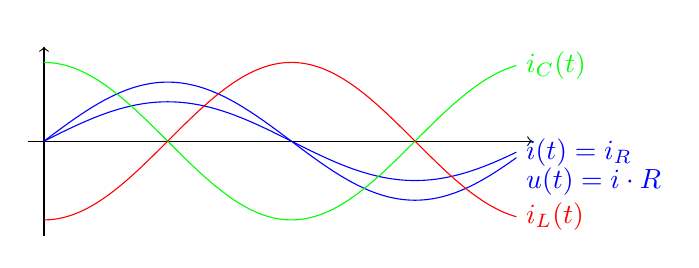
\begin{tikzpicture}[domain=0:6]
	
	\draw[->] (-0.2,0) -- (6.2,0) node[right] {};
	\draw[->] (0,-1.2) -- (0,1.2) node[above] {};
	\draw[color=blue, samples=150]   plot (\x,{0.5*sin(\x r)})   node[right]
	{$i(t)=i_R$};
	\draw[color=blue, samples=150]   plot (\x,{0.75*sin(\x r)})   node[below right]
	{$u(t)=i\cdot R$};
	\draw[color=green, samples=150]   plot (\x,{cos(\x r)})   node[right]
	{$i_C(t)$};
	\draw[color=red, samples=150]   plot (\x,{-1*cos(\x r)})  
	node[right] {$i_L(t)$};
\end{tikzpicture} 
	\label{fig:schwingkreise:erzwungener:sinus} 
}
\caption{Erzwungener Schwingkreis}
\label{fig:schwingkreise:erzwungene}
\end{figure}

\begin{figure}[!h]
	\centering
	\pgfmathdeclarefunction{gauss}{2}{%
  \pgfmathparse{1/(#2*sqrt(2*pi))*exp(-((x-#1)^2)/(2*#2^2))}%
}

\makebox{\begin{tikzpicture}[scale=0.7, every node/.style={scale=1.3}]
\begin{axis}[
  no markers,
  domain=0:6,
  samples=500,
  hide x axis=true,
	hide y axis=true,
  %height=5cm, width=12cm,
  %xtick={4,6.5}, ytick=\empty,
  enlargelimits=false,
  clip=false,
  axis on top,
  grid = major
  ]
  \addplot {gauss(3,1)};
\end{axis}

	\draw[->, thick] (-0.2,0) -- +(right:7.5) node[right] {$t$};
	\draw (3.43,0) node[anchor=north] {$\omega_r$};
		\draw[dashed] (3.43,0) -- +(0,6);
	\draw (2.43,0) node[anchor=north] {$\omega_1$};
	\draw (4.43,0) node[anchor=north] {$\omega_2$};

	\draw[->, thick] (0,-0.2) -- +(north:6.5) node[above] {$\underline{Z}$};
	\draw (0.05,3.85) -- (-0.05,3.85) node[anchor=east] {$\frac{R}{\sqrt{2}}$};
	\draw (0.05,5.7) -- (-0.05,5.7) node[anchor=east] {$R$};

	\draw[dashed] (0,3.85) -- (4.5,3.85);
	\draw[dashed] (0,5.7) -- (3.55,5.7);
	\draw[dashed, shorten <= -3pt,] (2.43,4) -- (2.43,0);
	%\draw[dashed, shorten <= -3pt] (3.43,5.75) -- (3.43,0);
	\draw[dashed, shorten <= -3pt] (4.43,4) -- (4.43,0);
	\draw[<->] (4.5,4) -- (4.5,5.75) node[below right] {$3dB$};


\end{tikzpicture}}

	\caption{t-Z-Diagramm mit 3dB Punkten}
	\label{fig:tZDiagramm}
\end{figure}



Resonanz: $\omega = \omega_r$\\
\begin{align}
	\underline{Y}_C +\underline{Y}_L &= 0\nonumber\\
	j\omega C+\frac{1}{j\omega L} &= 0\nonumber\\
	\omega=\omega_r&=\frac{1}{\sqrt{LC}}\nonumber\\
	I_C&=U\cdot\omega_rC=I\cdot R \cdot \omega_rC=I\cdot R
	\frac{C}{\sqrt{LC}}\nonumber\\
	&=I\cdot R \sqrt{\frac{C}{L}} = I \cdot Q\nonumber\\
	I_L&=\frac{U}{\omega_rL}=I \cdot Q\nonumber\\
	\omega_r&=\frac{1}{\sqrt{LC}}\nonumber\\
	\frac{f_r}{\Delta f}=\frac{\omega_r}{\Delta \omega} &= Q\nonumber
\end{align}\\


  
\subsubsection{Parallelschwingkreis}
$$\underline{Z} = \frac{1}{\frac{1}{j\omega L}+\frac{1}{R} + j \omega C}
= \frac{j\omega L}{1+j\omega \frac{L}{R}+(j\omega)^2LC}
= \frac{R}{1+(\frac{1}{j\omega L}+j\omega C)R}$$\\
normiert:\\
\begin{align}
\frac{\underline{Z}}{R}&=\frac{1}{1+j(\omega C-\frac{1}{\omega L})\cdot R}
=\frac{j\omega \frac{L}{R}}{1+j\omega\frac{L}{R}+(j\omega)^2LC}\nonumber\\
&=\frac{1}{\sqrt{1+(\omega C - \frac{1}{\omega
L})^2R^2}} \angle \arctan{((\frac{1}{\omega L}-\omega C)\cdot R)} \nonumber
\end{align}\\

Frequenzgang von $\underline Z$:\\
\begin{align}
	\text{Spez. Pt.}&&
	\operatorname{Im}{\{Z\}} = 0 \rightarrow \omega =
	\omega_r=\frac{1}{\sqrt{LC}}\nonumber\\ && Z = Z_{max} = R\nonumber\\
	\text{Tiefe Frequenzen} &&
	\omega \ll \omega_r: \frac{\underline Z}{R} \approx
	j\omega\frac{L}{R}=\omega\frac{L}{R} \angle +90^\circ induktiv\nonumber\\ && \omega \gg \omega_r: \frac{\underline Z}{R} \approx \frac{1}{j\omega RC}
	\angle -90^\circ kapazitiv\nonumber\\
	\text{3dB-Pt} &&
	\frac{Z}{R}=\frac{1}{\sqrt{2}}\nonumber\\
	&& \frac{1}{1+(\omega C-\frac{1}{\omega L})^2R^2}=\frac{1}{2}\nonumber
\end{align}\\

% \begin{wrapfigure}{l}{0.5\textwidth}
% 	\centering
% 	\pgfmathdeclarefunction{gauss}{2}{%
  \pgfmathparse{1/(#2*sqrt(2*pi))*exp(-((x-#1)^2)/(2*#2^2))}%
}

\makebox{\begin{tikzpicture}[scale=0.7, every node/.style={scale=1.3}]
\begin{axis}[
  no markers,
  domain=0:6,
  samples=500,
  hide x axis=true,
	hide y axis=true,
  %height=5cm, width=12cm,
  %xtick={4,6.5}, ytick=\empty,
  enlargelimits=false,
  clip=false,
  axis on top,
  grid = major
  ]
  \addplot {gauss(3,1)};
\end{axis}

	\draw[->, thick] (-0.2,0) -- +(right:7.5) node[right] {$t$};
	\draw (3.43,0) node[anchor=north] {$\omega_r$};
		\draw[dashed] (3.43,0) -- +(0,6);
	\draw (2.43,0) node[anchor=north] {$\omega_1$};
	\draw (4.43,0) node[anchor=north] {$\omega_2$};

	\draw[->, thick] (0,-0.2) -- +(north:6.5) node[above] {$\underline{Z}$};
	\draw (0.05,3.85) -- (-0.05,3.85) node[anchor=east] {$\frac{R}{\sqrt{2}}$};
	\draw (0.05,5.7) -- (-0.05,5.7) node[anchor=east] {$R$};

	\draw[dashed] (0,3.85) -- (4.5,3.85);
	\draw[dashed] (0,5.7) -- (3.55,5.7);
	\draw[dashed, shorten <= -3pt,] (2.43,4) -- (2.43,0);
	%\draw[dashed, shorten <= -3pt] (3.43,5.75) -- (3.43,0);
	\draw[dashed, shorten <= -3pt] (4.43,4) -- (4.43,0);
	\draw[<->] (4.5,4) -- (4.5,5.75) node[below right] {$3dB$};


\end{tikzpicture}}

% 	\caption{3dB-Punkt}
% 	\label{fig:3dBPunkt}
% \end{wrapfigure}


\begin{align}
	(\omega C-\frac{1}{\omega L})^2R^2 &= 1\nonumber\\
	(\omega C - \frac{1}{\omega L})R &= \pm 1\nonumber\\
	\omega C - \frac{1}{\omega L} &= \pm \frac{1}{R}\nonumber\\
	\omega^2 \pm \omega \frac{1}{RC}-\frac{1}{LC} &= 0\nonumber\\
	\omega^2 + \frac{\omega_r}{Q}\cdot \omega - \omega_r^2&=0 \\ bzw\\ \omega^2 -
	\frac{\omega_r}{Q}\cdot \omega - \omega_r^2=0\nonumber
	\omega_{1,1,2} = -\frac{\omega_r}{2Q} \pm 
	\underbrace{\omega_r\sqrt{\frac{1}{4Q^2}+1}}_{>\frac{\omega_r}{2Q}}
	\\	bzw \\
	\omega_{2,1,2}=\frac{\omega_r}{2Q} \pm
	\underbrace{\omega_r\sqrt{\frac{1}{4Q^2}+1}}_{>\frac{\omega_r}{2Q}} \nonumber\\
\end{align}
%geschwoffene klammern unten dran mechen //TODO


3dB Frequenzgrenzen:\\
\begin{align}
\boxed{\omega_{1,2}=\omega_r(\sqrt{\frac{1}{4Q^2}+1}\mp\frac{1}{2Q})}
\end{align}

